\documentclass[11pt]{article}
\usepackage[margin=1in]{geometry}
\usepackage{lmodern}
\usepackage[T1]{fontenc}
\usepackage{amsmath,amssymb}
\usepackage{booktabs}
\usepackage{graphicx}
\usepackage{url}
\setlength{\parskip}{0.4em}
\setlength{\parindent}{0pt}
\renewcommand{\arraystretch}{1.15}
\setlength{\tabcolsep}{4.5pt}

\title{\vspace{-1.2cm}\textbf{Ternary Anchoring Lookup Tables}}
\author{Anatoly Starostin \\ DeepSpike Inc.}
\date{Draft --- \today}

\begin{document}
\maketitle
\vspace{-0.8cm}

\begin{abstract}
\noindent Ternary Anchoring Lookup Tables (TALUT) replace the input-side routing of a
lookup-table (LUT) FFN with sign-tests against learned hyperplanes whose coefficients are
ternary, $\{-1,0,+1\}$. This generalises the anchor-pair comparison of the basic table while
keeping the index-and-gather forward unchanged, and it removes the input-side matmul: at
deployment, with precomputed indices, the FFN block reduces to a table gather plus an optional
output-decompress. On a short-context language-modelling benchmark a TALUT FFN reaches bpb
$1.18943$ at $76.4$M parameters, below the vanilla MLP baseline ($1.20144$), with a
multiplication-free deployed routing. We give the training relaxation, the deployment-cost
accounting, a forced-sparsity study, and a $16$k-step sweep. We are explicit about scope: ternary
routing does \emph{not} beat a dense \texttt{bf16} GEMM on a GPU; it is of interest only under
specialised hardware that benefits from the absence of multiplications, and only away from the
high-sparsity regime that both costs bpb and collapses back toward anchor pairs. All code is
available at \url{https://github.com/anatoli-starostin/spiky}.
\end{abstract}

\section{Introduction and scope}
\label{sec:intro}
This paper is a focused study of one way to build the lookup-table FFN of~\cite{manifesto}: making
the per-table routing multiplication-free. The surrounding programme --- replacing the transformer
FFN by lookup tables at matched language-modelling quality, and the non-ternary routes to it
(dynamic decompression, input reprojection) --- is reported separately; here we take the
lookup-table FFN as given (recalled in Section~\ref{sec:basic}) and study the ternary hyperplane
routing on its own.

\paragraph{Scope and hardware assumption.} It is worth being precise about when the ternary
construction helps. Keeping the routing coefficients in $\{-1,0,+1\}$ removes multiplications from
the input-side projection, but on current GPU hardware this is not by itself an advantage: a dense
\texttt{bf16} GEMM is extremely fast and heavily optimised, and a multiplication-free
add/subtract routing does not beat it at equal work. The only regime in which ternary routing wins
is under \emph{very high sparsity} --- few non-zero coefficients per hyperplane, so the projection
touches only a handful of coordinates. But, as Section~\ref{sec:sparsity} shows, forcing that
sparsity costs bpb monotonically, and in the sparse limit the general ternary hyperplane collapses
back toward the original anchor-pair comparison (two non-zeros). We therefore frame the paper under
an explicit assumption: ternary/multiplication-free routing is of interest for \emph{specialised
hardware} that strongly benefits from the absence of multiplications (and reads only selected
table rows), not for a commodity GPU running dense \texttt{bf16} matmuls. Under that assumption the
deployment-cost accounting of Section~\ref{sec:deploy} is the relevant metric; on a GPU it is not.

\section{Background: the lookup-table FFN}
\label{sec:basic}
We replace the FFN of each transformer block by a multi-table lookup. For an input
$x\in\mathbb{R}^{d}$, each table $t$ computes a $k$-bit index from $k$ binary tests and gathers one
stored row; the block output is the sum over tables,
\begin{equation}
\label{eq:lutfwd}
\mathrm{idx}_t(x)=\sum_{j} 2^{\,j-1}\,\mathbf{1}\!\left[\langle q_{tj},x\rangle+b_{tj}>0\right],
\qquad
\mathrm{LUT}(x)=\sum_t W_t\!\left[\mathrm{idx}_t(x)\right].
\end{equation}
In the basic table of~\cite{manifesto} each test is an \emph{anchor-pair} comparison
$\mathbf{1}[x_{a_j}>x_{b_j}]=\mathbf{1}[\langle q_j,x\rangle>0]$ with $q_j=e_{a_j}-e_{b_j}$, i.e.\ a
hyperplane with exactly one $+1$ and one $-1$. The index is a step function of $x$, so the forward
is a hard, non-differentiable comparison; training uses a hard-forward / soft-backward scheme in
which the anchor comparison is relaxed by a rational soft-sign of the margin $x_{a}-x_{b}$ (and a
per-table temperature), while the gathered rows $W_t$ are ordinary trainable parameters.

\paragraph{Metrics.} We report validation bits-per-byte (bpb), FLOPs, and \emph{virtual
bandwidth} (vBW). FLOPs is the per-token forward arithmetic of the FFN block, counted
conservatively: the output decompression matmul, if present (each multiply-add as two FLOPs),
plus one FLOP for each hyperplane sign test and one FLOP for each addition in the projection and
the gather-and-sum. A ternary $\{-1,0,+1\}$ coefficient is a sign-flip or a skip, not a real
multiply, so a nonzero coefficient contributes one add and a zero contributes nothing: the
projection $\langle q,x\rangle$ costs one FLOP per nonzero coefficient of $q$. vBW is the
decode-regime bytes per token, with LUT tables read as selected rows only (a specialised-hardware
assumption). The reference point is an untied vanilla $4\times$ MLP FFN at $1.20144$ bpb
($35.79$M parameters), whose dense FFN block costs $14.16$M FLOPs and $14.16$M vBW per token. A
strong non-ternary LUT configuration, the input-reprojection anchor exp\_n\_0121 ($H4$, $d48$,
nap8, tph128), reaches $1.19142$ bpb at $67.4$M parameters with an FFN block of $1.94$M FLOPs /
$2.07$M vBW, at the cost of an input-side reprojection matmul. TALUT starts from that
configuration and removes the matmul.

\section{Ternary Anchoring Lookup Tables}
\label{sec:talut}
Input reprojection routes each table in a small learned subspace at the cost of an input-side
matmul. Ternary Anchoring Lookup Tables (TALUT) keep the same index-and-gather machinery of
Eq.~\eqref{eq:lutfwd} yet remove that matmul, by generalising the anchor-pair comparison itself.

\paragraph{Correspondence to the basic LUT.} TALUT reuses the forward of
Section~\ref{sec:basic} unchanged: the $k$-bit index and the summed gather
$\mathrm{LUT}(x)=\sum_t W_t[\mathrm{idx}_t(x)]$ are identical. Only the per-bit test changes. In the
basic LUT bit $j$ is the anchor-pair comparison
\begin{equation}
\mathbf{1}\!\left[x_{a_{j}}>x_{b_{j}}\right]
\;=\;\mathbf{1}\!\left[\langle q_{j},x\rangle>0\right],\qquad q_{j}=e_{a_{j}}-e_{b_{j}},
\end{equation}
i.e.\ a hyperplane whose coefficient vector $q_{j}\in\{-1,0,+1\}^{d}$ has exactly one $+1$
(at $a_{j}$) and one $-1$ (at $b_{j}$). TALUT lets $q_{j}$ be \emph{any} ternary vector in
$\{-1,0,+1\}^{d}$ and adds a threshold $b_{j}$:
\begin{equation}
\mathbf{1}\!\left[\langle q_{j},x\rangle+b_{j}>0\right],\qquad q_{j}\in\{-1,0,+1\}^{d}.
\end{equation}
The anchor pair is the special case (one $+1$, one $-1$, the rest zero); a general ternary
hyperplane is strictly more expressive, and its projection still needs no multiplications ---
only additions and subtractions of the selected coordinates plus one threshold compare.

\paragraph{Training.} The ternary coefficients are the hard ternarisation of real shadow
weights $w\in\mathbb{R}^{d}$ (one per hyperplane), relaxed by a straight-through quantiser
with a single temperature $T$ per table:
\begin{equation}
s=\tanh\!\Big(\frac{w}{2T}\Big),\qquad
q_{\mathrm{hard}}=\begin{cases}+1 & s>\tfrac12\\ -1 & s<-\tfrac12\\ 0 & \text{otherwise}\end{cases},\qquad
q=s+\big(q_{\mathrm{hard}}-s\big).\mathrm{detach()} .
\end{equation}
The forward value is exactly ternary; the gradient flows through the smooth $s$ to $w$ and to
$\log T$. The dead zone has the closed form $q=0\Leftrightarrow|w|\le T\ln 3$, so $T$ is
literally the width of the zero band in weight units: small $T$ drives coefficients to
$\pm1$, large $T$ to $0$. A trainable per-hyperplane bias $b$ supplies the threshold above
(it survives to deployment as a comparison threshold, not a coefficient, so inference stays
multiplication-free), and the projection is normalised so that no free scale parameter is
needed. The shadow weights $w$ are discarded after training; the deployed routing stores only
the ternary coefficients (two bits per entry) and the bias thresholds.

\paragraph{Backward, in parallel to the basic LUT.} Both routings make a hard, non-differentiable
comparison trainable, and the relaxation is where they differ. The basic LUT
(Section~\ref{sec:basic}) relaxes the anchor comparison by a rational soft-sign of the margin
$x_{a}-x_{b}$; TALUT relaxes the ternary quantisation of the coefficients by the $\tanh$
straight-through $s=\tanh(w/2T)$ over the shadow weights, while the sign of the pre-activation
$\langle q,x\rangle+b$ is relaxed by the same soft-score surrogate the basic LUT uses. So the
trainable degree of freedom moves from the fixed anchor indices (the basic LUT trains only the
temperature and the table rows) to the hyperplane coefficients themselves.

\subsection{Deployment cost}
\label{sec:deploy}
The routing indices could be precomputed at deployment, but under the conservative convention we
count the ternary routing as if it were computed. Each hyperplane then costs one add per nonzero
coefficient of $\langle q,x\rangle$ plus one sign test, the gather-and-sum adds one FLOP per
summed element, and the output-decompress matmul, where present, adds its multiply-adds. The
projection over the nonzero coefficients dominates: for the anchor exp\_n\_0134 (per-head
decompress, about $172$ nonzero coefficients per hyperplane) the FFN block is about $5.3$M FLOPs,
so removing the input-side matmul does not by itself make the block FLOP-cheap. The count falls
toward about $2$M as the routing is forced sparser (Section~\ref{sec:sparsity}) or the head count
is reduced, and rises above the dense $14.16$M for the densest, widest configurations. Virtual
bandwidth is unaffected by this accounting: the block reads only its selected rows, about $2.4$M
(no decompression) or $\approx 1.2$M (decompression) bytes per token, against the dense MLP FFN's
$14.16$M.

\subsection{Forced sparsity}
\label{sec:sparsity}
The temperature $T$ already sets the width of the ternary dead
zone ($|w|\le T\ln 3$); at the max-entropy $T$ roughly one third of the coefficients are zero.
To push the routing sparser than that --- fewer non-zero $\pm1$ components per hyperplane, and
hence cheaper add/subtract routing --- we add an explicit penalty. The penalty acts on a smooth
surrogate for the non-zero fraction: the mean over all hyperplane weight elements of
$|s_i|=|\tanh(w_i/2T)|$, the same $\mathrm{stanh}$ the routing uses. With a target non-zero
fraction $f^{\star}$ (a target count of non-zeros per hyperplane divided by the input dimension
$d$), the loss is a one-sided hinge with weight $\lambda$, summed over the LUT modules:
\begin{equation}
\mathcal{L}_{\mathrm{sparse}}\;=\;\lambda\,\operatorname{ReLU}\!\Big(\tfrac{1}{N}\textstyle\sum_{i} \big|\tanh(w_i/2T)\big|\;-\;f^{\star}\Big).
\end{equation}
It applies full pressure while the soft non-zero fraction exceeds $f^{\star}$ and switches off at
or below it; the hinge is plain (not squared) so it holds full pressure right up to the target.
$T$ is detached inside the surrogate, so the penalty gradient reaches only the shadow weights.
The mean (rather than a sum) makes $\lambda$ scale-invariant across table shapes, and the
realised non-zero fraction is logged at every eval. With $\lambda=100$ and $f^{\star}$ set by
the target count (e.g.\ $192/384=0.5$), the hinge drives the routing well below its
unregularised density and then holds there. Figure~\ref{fig:sparsity} shows the per-step
trajectories for three
$4$k runs on one recipe ($H4$ per-head decompress, $76.4$M params): unregularised routing
settles at $269.0$ non-zero coefficients per hyperplane, the target-$192$ hinge at $161.6$, and
target-$64$ at $47.9$. The soft surrogate systematically undershoots the hard count --- $192$
maps to $161.6$ and $64$ to $47.9$ --- because the target is met on $\mathrm{stanh}$, which sits
below the true density; a wanted hard count cannot be obtained by scaling the target.

Forcing the routing sparser is not free at bpb, and this is already visible at $4$k: the three
runs worsen monotonically as the target tightens --- unregularised $1.34646$, target-$192$
$1.34841$, target-$64$ $1.36521$ validation bpb --- so every increment of enforced sparsity
costs modelling quality. The hinge earns its keep in the deployment-time density it buys (fewer
non-zero add/subtract components per hyperplane), not in a bpb gain; the full-anneal 16k sweep
below shows the same monotone cost.

\begin{figure}[h]\centering
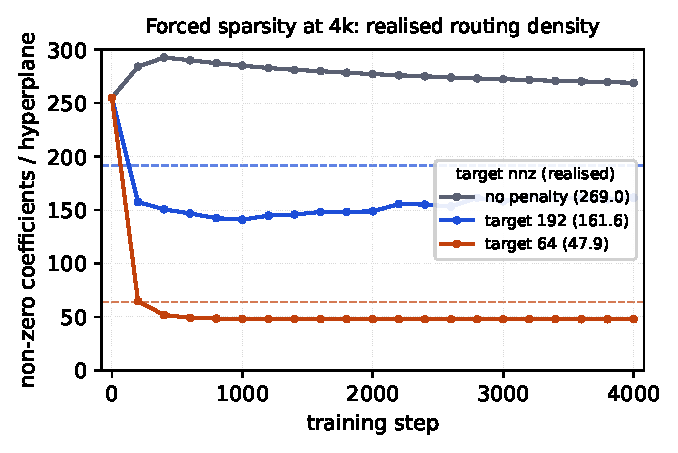
\includegraphics[width=0.62\linewidth]{sparsity_fig.pdf}
\caption{Realised routing density over training for three $4$k runs (\texttt{exp\_g\_0037}
unregularised, \texttt{exp\_g\_0044} target $192$, \texttt{exp\_g\_0042} target $64$), read from
each run's per-step \texttt{nonzero\_per\_hyperplane} log. Dashed lines mark the two hinge
targets. Each hinge reaches its regime within a few hundred steps and holds, settling below the
nominal target on the hard non-zero count.}
\label{fig:sparsity}
\end{figure}

\section{16k-step results}
\label{sec:results}
Applying TALUT to the input-reprojection anchor exp\_n\_0121
($H4$, $d48$, nap8, tph128; $1.19142$ bpb) replaces its learned reprojection matmul with
ternary gather-and-sum and reaches bpb $1.18943$ (exp\_n\_0134, $76.4$M), below the vanilla
baseline. The bpb drop is small, and the point of the change is that inference becomes
multiplication-free, not that it saves FLOPs. Under the conservative count the removed
reprojection matmul is small next to the ternary projection over the routing coefficients, so at
the anchor the FFN block is about $5.3$M FLOPs rather than the reprojection form's $1.94$M, at
$1.18$M vBW. Table~\ref{tab:sweep} reports a one-axis-at-a-time sweep around this anchor. All are
the per-head output-decompress form ($H$ heads of inner width $48$, concatenated to
$H\!\cdot\!48=192$ and decompressed to $384$). The FFN FLOPs vary across the sweep, since the
projection over the nonzero coefficients dominates, so more heads, more anchor pairs, and denser
routing all raise it, from about $2$M to about $14$M; the selected-row virtual bandwidth is
$\approx1.18$M per token wherever $\mathrm{tph}=128$ (the head, sparsity, and anchor-pair axes all
hold it there) and changes only along the tables-per-head axis ($1.03$M at tph64, $2.06$M at
tph256).

\begin{table}[ht]\centering
\begin{tabular}{llrrll}
\toprule
run & variant & bpb & params & FFN FLOPs\,/\,vBW & $\Delta$ vs 0134 \\
\midrule
exp\_n\_0147 & $H4$, out48, tph256 & \textbf{1.18187} & 123.6M & 9.68M / 2.06M & $-0.00756$ \\
exp\_n\_0149 & $H8$, out24, no penalty & 1.18203 & 85.8M & 14.26M / 1.18M & $-0.00740$ \\
exp\_n\_0145 & $H4$, out48, nap10 & 1.18296 & 192.0M & 6.35M / 1.18M & $-0.00647$ \\
exp\_n\_0143 & $H8$, out24, target 192 & 1.18483 & 85.8M & 9.54M / 1.18M & $-0.00460$ \\
exp\_n\_0141 & $H4$, out48, no penalty & 1.18757 & 76.4M & 7.64M / 1.18M & $-0.00186$ \\
exp\_n\_0140 & $H4$, out48, target 256 & 1.18851 & 76.4M & 6.34M / 1.18M & $-0.00092$ \\
exp\_n\_0134 & $H4$, out48, target 192 (anchor) & 1.18943 & 76.4M & 5.29M / 1.18M & $0$ \\
exp\_n\_0142 & $H2$, out96, target 192 & 1.19583 & 71.6M & 3.16M / 1.18M & $+0.00640$ \\
exp\_n\_0144 & $H4$, out48, nap6 & 1.19694 & 45.7M & 4.22M / 1.18M & $+0.00751$ \\
exp\_n\_0150 & $H1$, out192, target 192 & 1.20011 & 69.3M & 2.08M / 1.18M & $+0.01068$ \\
exp\_n\_0139 & $H4$, out48, target 128 & 1.20460 & 76.4M & 3.14M / 1.18M & $+0.01517$ \\
exp\_n\_0146 & $H4$, out48, tph64 & 1.20600 & 52.8M & 3.08M / 1.03M & $+0.01657$ \\
exp\_n\_0148 & $H4$, out48, target 64 & 1.20942 & 76.4M & 2.23M / 1.18M & $+0.01999$ \\
\bottomrule
\end{tabular}
\caption{16k ternary sweep around exp\_n\_0134 ($\Delta$ vs its $1.18943$). Steps $16{,}000$ and
batch $24{,}576$ throughout (omitted). FFN FLOPs use the conservative convention (one add per
nonzero routing coefficient), so they scale with the realised nonzero density per hyperplane
(committed for exp\_n\_0134 at $172$, exp\_n\_0149 at $268$, exp\_n\_0150 at $170$; the other
target-$192$ rows use $\approx172$, no-penalty $\approx268$, and the target-$128$/$256$/$64$ rows
their realised densities). vBW is unchanged and varies only along the tables-per-head axis. The
sweep-best in bpb is exp\_n\_0147 (tph256, $1.18187$).}
\label{tab:sweep}
\end{table}

All three swept axes read cleanly. \textbf{Head count (axis A): more, narrower heads win.} bpb is
monotone in $H$ at fixed budget (all at target 192) --- $H8$ ($1.18483$) $<H4$ ($1.18943$) $<H2$
($1.19583$) $<H1$ ($1.20011$, exp\_n\_0150).
\textbf{Sparsity target (axis C): denser is better.} bpb is monotone in the forced non-zero
count: no penalty ($1.18757$) $<$ target 256 ($1.18851$) $<$ target 192 ($1.18943$) $<$ target
128 ($1.20460$) $<$ target 64 ($1.20942$); so at the full 16k budget the sparsity hinge is a real
quality cost, the same monotone degradation already seen at $4$k (Figure~\ref{fig:sparsity}).
\textbf{LUT size (axis B): bigger tables win.} bpb is monotone in both size knobs --- in cells
(nap6 $1.19694$ $<$ nap8 $1.18943$ $<$ nap10 $1.18296$) and in tables per head (tph64 $1.20600$
$<$ tph128 $1.18943$ $<$ tph256 $1.18187$) --- so a larger table budget keeps improving bpb, at a
rising parameter cost (and, for the tables axis, a rising bandwidth cost). The sweep-best is the
tph256 run exp\_n\_0147 ($1.18187$, $123.6$M). The axes combine: stacking axis-A's $H8$ with
axis-C's no penalty (exp\_n\_0149, $H8$ + no penalty) reaches $1.18203$, nearly tying the
sweep-best tph256 run (exp\_n\_0147, $1.18187$) but not beating it --- so the head and sparsity
gains do stack; combining them further with more tables/cells is the natural next config.
Figure~\ref{fig:ternary} lays the sweep out along its swept axes: parameters (panel a, coloured by
axis), the sparsity target (panel b), and the head count (panel c); the anchor exp\_n\_0134 is the
gold star and the dashed line is the vanilla baseline.

\begin{figure}[ht]\centering
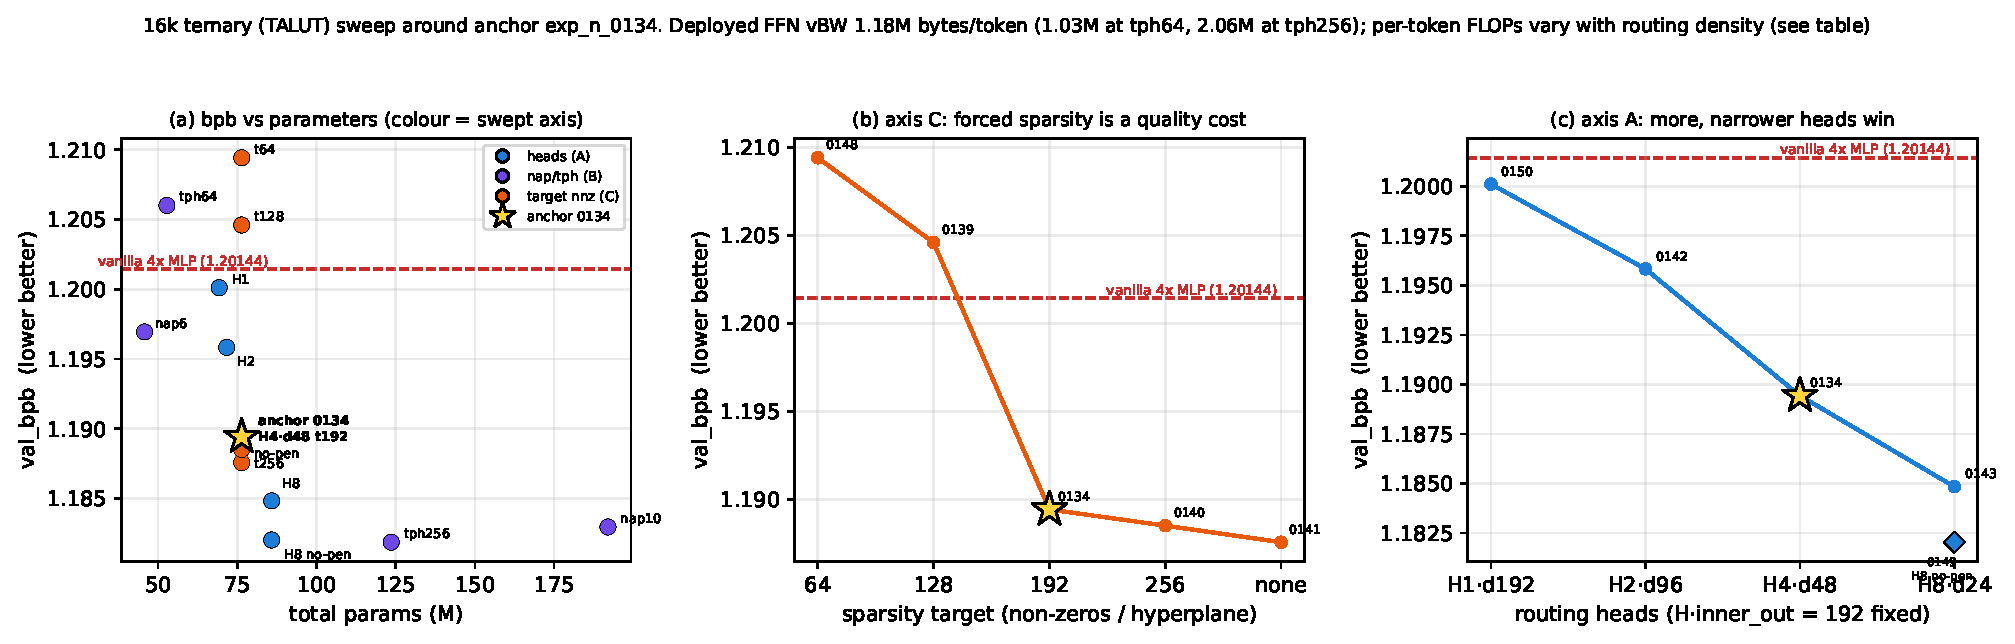
\includegraphics[width=\linewidth]{ternary_sweep_fig.pdf}
\caption{16k ternary (TALUT) sweep around anchor exp\_n\_0134 (gold star), all thirteen runs.
(a) validation bpb against total parameters, coloured by the swept axis --- head count (A),
nap/tables (B), sparsity target (C); (b) the sparsity axis, bpb against the forced non-zero
target ($64\to256$, then no penalty); (c) the head-count axis at fixed $H\!\cdot\!\text{inner\_out}=192$.
The dashed line is the untied vanilla baseline ($1.20144$). Lower is better on every bpb axis.}
\label{fig:ternary}
\end{figure}

\section{Conclusion}
\label{sec:conclusion}
Generalising the anchor-pair comparison of a lookup-table FFN to a ternary hyperplane sign-test
removes the input-side matmul while keeping the index-and-gather forward unchanged. On a
short-context benchmark the resulting TALUT FFN matches the vanilla MLP's bpb at $76.4$M
parameters ($1.18943$ vs $1.20144$), and at deployment, with precomputed indices, the FFN block's
routing is multiplication-free and it reads only its selected rows, though under the conservative
count it still costs a few million FLOPs (about $5.3$M at the anchor, ranging from about $2$M to
about $14$M across the sweep), not zero. Forced sparsity is a
real quality cost, monotone in the enforced non-zero count at both $4$k and $16$k, so density is
bought against bpb rather than for free. The whole construction is worth stating under its
assumption: on a commodity GPU a dense \texttt{bf16} GEMM already wins, and the ternary,
multiplication-free routing is of interest only for specialised hardware that benefits from the
absence of multiplications. The sweep is now complete: its best point is the tables-per-head run
exp\_n\_0147 (tph256, $1.18187$), and stacking two axis-winners --- $H8$ with no penalty
(exp\_n\_0149, $1.18203$) --- nearly ties it, so combining the head, sparsity, and table-size
gains further is the natural next config, at higher parameter cost.

\vspace{0.5em}
\hrule
\vspace{0.4em}
{\footnotesize All runs are on branch research/hyperplane\_ffn\_next. FLOPs are forward
multiply-adds per token; virtual bandwidth is decode-regime bytes per token with LUT tables
read as selected rows only (specialised-hardware assumption). Ternary FLOPs/vBW are on the
deployed basis with precomputed indices.}

\begin{thebibliography}{9}
\bibitem{manifesto} E.~M.~Izhikevich.
``Spiking Manifesto.''
arXiv:2512.11843, December 2025.
\bibitem{nanochat} A.~Karpathy. ``nanochat: a minimal full-stack ChatGPT-style pipeline.''
Software, 2025. \texttt{https://github.com/karpathy/nanochat}.
\bibitem{ltcb} M.~Mahoney. ``Large Text Compression Benchmark.'' Online, 2011.
\texttt{http://mattmahoney.net/dc/text.html}.
\end{thebibliography}

\end{document}
